\hypertarget{sec-feature-selection}{%
\chapter{Feature Selection}\label{sec-feature-selection}}

\vspace{-15mm}\addtocontents{toc}{\textit{Marvin N. Wright}}

\textbf{Marvin N. Wright} \newline  \emph{Leibniz Institute for
Prevention Research and Epidemiology -- BIPS, and University of Bremen,
and University of Copenhagen} \newline \newline 

Feature selection\index{feature selection}, also known as variable or
descriptor
selection\index{variable selection|see{feature selection}}\index{descriptor selection|see{feature selection}},
is the process of finding a subset of features to use with a given task
and learner. Using an \emph{optimal set} of features can have several
benefits:

\begin{itemize}
\tightlist
\item
  improved predictive performance, since we reduce overfitting on
  irrelevant features,
\item
  robust models that do not rely on noisy features,
\item
  simpler models that are easier to interpret,
\item
  faster model fitting, e.g.~for model updates,
\item
  faster prediction, and
\item
  no need to collect potentially expensive features.
\end{itemize}

However, these objectives will not necessarily be optimized by the same
set of features and thus feature selection can be seen as a
multi-objective optimization\index{multi-objective optimization}
problem. In this chapter, we mostly focus on feature selection as a
means of improving predictive performance, but also briefly cover the
optimization of multiple criteria (Section~\ref{sec-multicrit-featsel}).

Reducing the number of features can improve models across many
scenarios, but it can be especially helpful in datasets that have a high
number of features in comparison to the number of data points. Many
learners perform implicit, also called embedded, feature
selection,\index{feature selection!implicit}\index{feature selection!embedded}
e.g.~via the choice of variables used for splitting in a decision tree.
Most other feature selection methods are model agnostic, i.e.~they can
be used together with any learner. Of the many different approaches to
identifying relevant features, we will focus on two general concepts,
which are described in detail below: Filter and Wrapper methods (Guyon
and Elisseeff 2003; Chandrashekar and Sahin 2014).

\hypertarget{sec-fs-filter}{%
\section{Filters}\label{sec-fs-filter}}

Filter methods are preprocessing\index{preprocessing} steps that can be
applied before training a model. A very simple filter approach could
look like this:

\begin{enumerate}
\def\labelenumi{\arabic{enumi}.}
\tightlist
\item
  calculate the correlation coefficient \(\rho\) between each feature
  and a numeric target variable, and
\item
  select all features with \(\rho > 0.2\) for further modeling steps.
\end{enumerate}

This approach is a \emph{univariate} filter because it only considers
the univariate relationship between each feature and the target
variable. Further, it can only be applied to regression tasks with
continuous features and the threshold of \(\rho > 0.2\) is quite
arbitrary. Thus, more advanced filter methods, e.g.~\emph{multivariate}
filters based on feature importance, usually perform better (Bommert et
al. 2020). On the other hand, a benefit of univariate filters is that
they are usually computationally cheaper than more complex filter or
wrapper methods. In the following, we describe how to calculate
univariate, multivariate and feature importance filters, how to access
implicitly selected features, how to integrate filters in a machine
learning pipeline and how to optimize filter thresholds.

Filter algorithms select features by assigning numeric scores to each
feature, e.g.~correlation between features and target variable, use
these to rank the features and select a feature subset based on the
ranking. Features that are assigned lower scores are then omitted in
subsequent modeling steps. All filters are implemented via the package
\href{https://mlr3filters.mlr-org.com}{\texttt{mlr3filters}}\index{\texttt{mlr3filters}}.
Below, we cover how to

\begin{itemize}
\tightlist
\item
  instantiate a
  \href{https://www.rdocumentation.org/packages/base/topics/funprog}{\texttt{Filter}}
  object,
\item
  calculate scores for a given task, and
\item
  use calculated scores to select or drop features.
\end{itemize}

Special cases of filters are feature
importance\index{feature importance} filters
(Section~\ref{sec-fs-var-imp-filters}) and embedded methods
(Section~\ref{sec-fs-embedded-methods}). Feature importance filters
select features that are important according to the model induced by a
selected
\href{https://mlr3.mlr-org.com/reference/Learner.html}{\texttt{Learner}}.
They rely on the learner to extract information on feature importance
from a trained model, for example, by inspecting a learned decision tree
and returning the features that are used as split variables, or by
computing model-agnostic feature importance
(Chapter~\ref{sec-interpretation}) values for each feature. Embedded
methods use the feature selection that is implicitly performed by some
learners and directly retrieve the internally selected features from the
learner.

\begin{tcolorbox}[enhanced jigsaw, opacitybacktitle=0.6, rightrule=.15mm, opacityback=0, arc=.35mm, breakable, titlerule=0mm, colframe=quarto-callout-tip-color-frame, coltitle=black, bottomrule=.15mm, toprule=.15mm, colback=white, colbacktitle=quarto-callout-tip-color!10!white, bottomtitle=1mm, toptitle=1mm, title=\textcolor{quarto-callout-tip-color}{\faLightbulb}\hspace{0.5em}{Independent Learners and Filters}, leftrule=.75mm, left=2mm]

The learner used in a feature importance or embedded filter is
independent of learners used in subsequent modeling steps. For example,
one might use feature importance of a random forest for feature
selection and train a neural network on the reduced feature set.

\end{tcolorbox}

Many filter methods are implemented in \texttt{mlr3filters}, including:

\begin{itemize}
\tightlist
\item
  Correlation, calculating Pearson or Spearman correlation between
  numeric features and numeric targets (\texttt{flt("correlation")})
\item
  Information gain, i.e.~mutual information of the feature and the
  target or the reduction of uncertainty of the target due to a feature
  (\texttt{flt("information\_gain")})
\item
  Minimal joint mutual information maximization (\texttt{flt("jmim")})
\item
  Permutation score, which calculates permutation feature importance
  (see Chapter~\ref{sec-interpretation}) with a given learner for each
  feature (\texttt{flt("permutation")})
\item
  Area under the ROC curve calculated for each feature separately
  (\texttt{flt("auc")})
\end{itemize}

Most of the filter methods have some limitations, for example, the
correlation filter can only be calculated for regression tasks with
numeric features. For a full list of all implemented filter methods, we
refer the reader to \url{https://mlr3filters.mlr-org.com}, which also
shows the supported task and features types. A benchmark of filter
methods was performed by Bommert et al. (2020), who recommend not to
rely on a single filter method but to try several ones if the available
computational resources allow. If only a single filter method is to be
used, the authors recommend to use a feature importance filter using
random forest permutation importance (see
(Section~\ref{sec-fs-var-imp-filters})), similar to the permutation
method described above, but also the JMIM and AUC filters performed well
in their comparison.

\hypertarget{sec-fs-calc}{%
\subsection{Calculating Filter Values}\label{sec-fs-calc}}

The first step is to create a new R object using the class of the
desired filter method. These are accessible from the
\href{https://mlr3filters.mlr-org.com/reference/mlr_filters.html}{\texttt{mlr\_filters}}\index{\texttt{mlr\_filters}}
dictionary with the sugar function
\href{https://mlr3filters.mlr-org.com/reference/flt.html}{\texttt{flt()}}\index{\texttt{flt()}}{\marginnote{\begin{footnotesize}\texttt{flt()}\end{footnotesize}}}.
Each object of class
\href{https://www.rdocumentation.org/packages/base/topics/funprog}{\texttt{Filter}}\index{\texttt{Filter}}
has a
\texttt{\$calculate()}\index{Filter!\$calculate()}{\marginnote{\begin{footnotesize}\texttt{\$calculate()}\end{footnotesize}}}
method, which computes the filter values and ranks them in a descending
order. For example, we can use the information gain filter described
above:

\begin{Shaded}
\begin{Highlighting}[]
\FunctionTok{library}\NormalTok{(mlr3filters)}
\NormalTok{flt\_gain }\OtherTok{=} \FunctionTok{flt}\NormalTok{(}\StringTok{"information\_gain"}\NormalTok{)}
\end{Highlighting}
\end{Shaded}

Such a \texttt{Filter} object can now be used to calculate the filter on
\texttt{tsk("penguins")} and get the results:

\begin{Shaded}
\begin{Highlighting}[]
\NormalTok{tsk\_pen }\OtherTok{=} \FunctionTok{tsk}\NormalTok{(}\StringTok{"penguins"}\NormalTok{)}
\NormalTok{flt\_gain}\SpecialCharTok{$}\FunctionTok{calculate}\NormalTok{(tsk\_pen)}

\FunctionTok{as.data.table}\NormalTok{(flt\_gain)}
\end{Highlighting}
\end{Shaded}

\begin{verbatim}
          feature    score
1: flipper_length 0.581168
2:    bill_length 0.544897
3:     bill_depth 0.538719
4:         island 0.520157
5:      body_mass 0.442880
6:            sex 0.007244
7:           year 0.000000
\end{verbatim}

This shows that the flipper and bill measurements are the most
informative features for predicting the species of a penguin in this
dataset, whereas sex and year are the least informative. Some filters
have hyperparameters that can be changed in the same way as
\texttt{Learner} hyperparameters. For example, to calculate
\texttt{"spearman"} instead of \texttt{"pearson"} correlation with the
correlation filter:

\begin{Shaded}
\begin{Highlighting}[]
\NormalTok{flt\_cor }\OtherTok{=} \FunctionTok{flt}\NormalTok{(}\StringTok{"correlation"}\NormalTok{, }\AttributeTok{method =} \StringTok{"spearman"}\NormalTok{)}
\NormalTok{flt\_cor}\SpecialCharTok{$}\NormalTok{param\_set}
\end{Highlighting}
\end{Shaded}

\begin{verbatim}
<ParamSet>
       id    class lower upper nlevels    default    value
1:    use ParamFct    NA    NA       5 everything         
2: method ParamFct    NA    NA       3    pearson spearman
\end{verbatim}

\hypertarget{sec-fs-var-imp-filters}{%
\subsection{Feature Importance Filters}\label{sec-fs-var-imp-filters}}

To use feature importance filters, we can use a learner with with an
\texttt{\$importance()} method that reports feature importance. All
learners with the property ``importance'' have this functionality. A
list of all learners with this property can be found with

\begin{Shaded}
\begin{Highlighting}[]
\FunctionTok{as.data.table}\NormalTok{(mlr\_learners)[}
  \FunctionTok{sapply}\NormalTok{(properties, }\ControlFlowTok{function}\NormalTok{(x) }\StringTok{"importance"} \SpecialCharTok{\%in\%}\NormalTok{ x)]}
\end{Highlighting}
\end{Shaded}

For some learners, the desired filter method needs to be set as a
hyperparameter. For example, \texttt{lrn("classif.ranger")} comes with
multiple integrated methods, which can be selected during construction:
To use the feature importance\index{feature importance} method
\texttt{"impurity"}, select it during learner construction:

\begin{Shaded}
\begin{Highlighting}[]
\FunctionTok{lrn}\NormalTok{(}\StringTok{"classif.ranger"}\NormalTok{)}\SpecialCharTok{$}\NormalTok{param\_set}\SpecialCharTok{$}\NormalTok{levels}\SpecialCharTok{$}\NormalTok{importance}
\end{Highlighting}
\end{Shaded}

\begin{verbatim}
[1] "none"               "impurity"           "impurity_corrected"
[4] "permutation"       
\end{verbatim}

\begin{Shaded}
\begin{Highlighting}[]
\NormalTok{lrn\_ranger }\OtherTok{=} \FunctionTok{lrn}\NormalTok{(}\StringTok{"classif.ranger"}\NormalTok{, }\AttributeTok{importance =} \StringTok{"impurity"}\NormalTok{)}
\end{Highlighting}
\end{Shaded}

We first have to remove missing data because the learner cannot handle
missing data, i.e.~it does not have the property ``missing''. Note we
use the \texttt{\$filter()} method presented in
Section~\ref{sec-tasks-mutators} here to remove rows; the ``filter''
name is unrelated to feature filtering, however.

\begin{Shaded}
\begin{Highlighting}[]
\NormalTok{tsk\_pen }\OtherTok{=} \FunctionTok{tsk}\NormalTok{(}\StringTok{"penguins"}\NormalTok{)}
\NormalTok{tsk\_pen}\SpecialCharTok{$}\FunctionTok{filter}\NormalTok{(tsk\_pen}\SpecialCharTok{$}\NormalTok{row\_ids[}\FunctionTok{complete.cases}\NormalTok{(tsk\_pen}\SpecialCharTok{$}\FunctionTok{data}\NormalTok{())])}
\end{Highlighting}
\end{Shaded}

Now we can use \texttt{flt("importance")} to calculate importance
values:

\begin{Shaded}
\begin{Highlighting}[]
\NormalTok{flt\_importance }\OtherTok{=} \FunctionTok{flt}\NormalTok{(}\StringTok{"importance"}\NormalTok{, }\AttributeTok{learner =}\NormalTok{ lrn\_ranger)}
\NormalTok{flt\_importance}\SpecialCharTok{$}\FunctionTok{calculate}\NormalTok{(tsk\_pen)}
\FunctionTok{as.data.table}\NormalTok{(flt\_importance)}
\end{Highlighting}
\end{Shaded}

\begin{verbatim}
          feature  score
1:    bill_length 76.164
2: flipper_length 50.032
3:     bill_depth 35.531
4:         island 24.880
5:      body_mass 22.422
6:            sex  1.419
7:           year  1.046
\end{verbatim}

\hypertarget{sec-fs-embedded-methods}{%
\subsection{Embedded Methods}\label{sec-fs-embedded-methods}}

Many learners internally select a subset of the features which they find
helpful for prediction, but ignore other features. For example, a
decision tree might never select some features for splitting. These
subsets can be used for feature selection, which we call embedded
methods\index{embedded methods} because the feature selection is
embedded in the learner. The selected features (and those not selected)
can be queried if the learner has the \texttt{"selected\_features"}
property. As above, we can find those learners with

\begin{Shaded}
\begin{Highlighting}[]
\FunctionTok{as.data.table}\NormalTok{(mlr\_learners)[}
  \FunctionTok{sapply}\NormalTok{(properties, }\ControlFlowTok{function}\NormalTok{(x) }\StringTok{"selected\_features"} \SpecialCharTok{\%in\%}\NormalTok{ x)]}
\end{Highlighting}
\end{Shaded}

For example, we can use \texttt{lrn("classif.rpart")}:

\begin{Shaded}
\begin{Highlighting}[]
\NormalTok{tsk\_pen }\OtherTok{=} \FunctionTok{tsk}\NormalTok{(}\StringTok{"penguins"}\NormalTok{)}
\NormalTok{lrn\_rpart }\OtherTok{=} \FunctionTok{lrn}\NormalTok{(}\StringTok{"classif.rpart"}\NormalTok{)}
\NormalTok{lrn\_rpart}\SpecialCharTok{$}\FunctionTok{train}\NormalTok{(tsk\_pen)}
\NormalTok{lrn\_rpart}\SpecialCharTok{$}\FunctionTok{selected\_features}\NormalTok{()}
\end{Highlighting}
\end{Shaded}

\begin{verbatim}
[1] "flipper_length" "bill_length"    "island"        
\end{verbatim}

The features selected by the model can be extracted by a
\href{https://www.rdocumentation.org/packages/base/topics/funprog}{\texttt{Filter}}
object, where \texttt{\$calculate()} corresponds to training the learner
on the given task:

\begin{Shaded}
\begin{Highlighting}[]
\NormalTok{flt\_selected }\OtherTok{=} \FunctionTok{flt}\NormalTok{(}\StringTok{"selected\_features"}\NormalTok{, }\AttributeTok{learner =}\NormalTok{ lrn\_rpart)}
\NormalTok{flt\_selected}\SpecialCharTok{$}\FunctionTok{calculate}\NormalTok{(tsk\_pen)}
\FunctionTok{as.data.table}\NormalTok{(flt\_selected)}
\end{Highlighting}
\end{Shaded}

\begin{verbatim}
          feature score
1:         island     1
2: flipper_length     1
3:    bill_length     1
4:     bill_depth     0
5:            sex     0
6:           year     0
7:      body_mass     0
\end{verbatim}

Contrary to other filter methods, embedded methods just return values of
\texttt{1} (selected features) and \texttt{0} (dropped feature).

\hypertarget{sec-fs-filter-based}{%
\subsection{Filter-Based Feature Selection}\label{sec-fs-filter-based}}

After calculating a score for each feature, one has to select the
features to be kept or those to be dropped from further modeling steps.
For the \texttt{"selected\_features"} filter described in embedded
methods (Section~\ref{sec-fs-embedded-methods}), this step is
straight-forward since the methods assign either a value of \texttt{1}
for a feature to be kept or \texttt{0} for a feature to be dropped.
Below, we find the names of features with a value of \texttt{1} and
select those features with \texttt{task\$select()}. At first glance it
may appear a bit convoluted to have a filter assign scores based on the
feature names returned by \texttt{\$selected\_features()}, only to turn
these scores back into the names of the features to be kept. However,
this approach allows us to use the same interface for all filter
methods, which is especially useful when we want to automate the feature
selection process in pipelines, as we will see in
Section~\ref{sec-pipelines-featsel}.

\begin{Shaded}
\begin{Highlighting}[]
\NormalTok{flt\_selected}\SpecialCharTok{$}\FunctionTok{calculate}\NormalTok{(tsk\_pen)}

\CommentTok{\# select all features used by rpart}
\NormalTok{keep }\OtherTok{=} \FunctionTok{names}\NormalTok{(}\FunctionTok{which}\NormalTok{(flt\_selected}\SpecialCharTok{$}\NormalTok{scores }\SpecialCharTok{==} \DecValTok{1}\NormalTok{))}
\NormalTok{tsk\_pen}\SpecialCharTok{$}\FunctionTok{select}\NormalTok{(keep)}
\NormalTok{tsk\_pen}\SpecialCharTok{$}\NormalTok{feature\_names}
\end{Highlighting}
\end{Shaded}

\begin{verbatim}
[1] "bill_length"    "flipper_length" "island"        
\end{verbatim}

For filter methods that assign continuous scores, there are essentially
two ways to select features:

\begin{itemize}
\tightlist
\item
  Select the top \(k\) features; or
\item
  Select all features with a score above a threshold \(\tau\).
\end{itemize}

The first option is equivalent to dropping the bottom \(p-k\) features.
For both options, one has to decide on a threshold, which is often quite
arbitrary. For example, to implement the first option with the
information gain filter:

\begin{Shaded}
\begin{Highlighting}[]
\NormalTok{tsk\_pen }\OtherTok{=} \FunctionTok{tsk}\NormalTok{(}\StringTok{"penguins"}\NormalTok{)}
\NormalTok{flt\_gain }\OtherTok{=} \FunctionTok{flt}\NormalTok{(}\StringTok{"information\_gain"}\NormalTok{)}
\NormalTok{flt\_gain}\SpecialCharTok{$}\FunctionTok{calculate}\NormalTok{(tsk\_pen)}

\CommentTok{\# select top three features from information gain filter}
\NormalTok{keep }\OtherTok{=} \FunctionTok{names}\NormalTok{(}\FunctionTok{head}\NormalTok{(flt\_gain}\SpecialCharTok{$}\NormalTok{scores, }\DecValTok{3}\NormalTok{))}
\NormalTok{tsk\_pen}\SpecialCharTok{$}\FunctionTok{select}\NormalTok{(keep)}
\NormalTok{tsk\_pen}\SpecialCharTok{$}\NormalTok{feature\_names}
\end{Highlighting}
\end{Shaded}

\begin{verbatim}
[1] "bill_depth"     "bill_length"    "flipper_length"
\end{verbatim}

Or, the second option with \(\tau = 0.5\):

\begin{Shaded}
\begin{Highlighting}[]
\NormalTok{tsk\_pen }\OtherTok{=} \FunctionTok{tsk}\NormalTok{(}\StringTok{"penguins"}\NormalTok{)}
\NormalTok{flt\_gain }\OtherTok{=} \FunctionTok{flt}\NormalTok{(}\StringTok{"information\_gain"}\NormalTok{)}
\NormalTok{flt\_gain}\SpecialCharTok{$}\FunctionTok{calculate}\NormalTok{(tsk\_pen)}

\CommentTok{\# select all features with score \textgreater{} 0.5 from information gain filter}
\NormalTok{keep }\OtherTok{=} \FunctionTok{names}\NormalTok{(}\FunctionTok{which}\NormalTok{(flt\_gain}\SpecialCharTok{$}\NormalTok{scores }\SpecialCharTok{\textgreater{}} \FloatTok{0.5}\NormalTok{))}
\NormalTok{tsk\_pen}\SpecialCharTok{$}\FunctionTok{select}\NormalTok{(keep)}
\NormalTok{tsk\_pen}\SpecialCharTok{$}\NormalTok{feature\_names}
\end{Highlighting}
\end{Shaded}

\begin{verbatim}
[1] "bill_depth"     "bill_length"    "flipper_length" "island"        
\end{verbatim}

In Section~\ref{sec-pipelines-featsel} we will return to filter-based
feature selection and how we can use pipelines\index{pipelines} and
tuning to automate and optimize the feature selection process.

\hypertarget{sec-fs-wrapper}{%
\section{Wrapper Methods}\label{sec-fs-wrapper}}

Wrapper methods work by fitting models on selected feature subsets and
evaluating their performance (Kohavi and John 1997). This can be done in
a sequential fashion, e.g.~by iteratively adding features to the model
in sequential forward selection, or in a parallel fashion, e.g.~by
evaluating random feature subsets in a random search. Below, we describe
these simple approaches in a common framework along with more advanced
methods such as genetic search. We further show how to select features
by optimizing multiple performance measures and how to wrap a learner
with feature selection to use it in pipelines or benchmarks.

In more detail, wrapper methods iteratively evaluate subsets of features
by resampling a learner restricted to this feature subset and with a
chosen performance metric (with holdout or a more expensive CV), and
using the resulting performance to guide the search. The specific search
strategy iteration is defined by a
\href{https://mlr3fselect.mlr-org.com/reference/FSelector.html}{\texttt{FSelector}}\index{\texttt{FSelector}}
object. A simple example is the sequential forward selection that starts
with computing each single-feature model, selects the best one, and then
iteratively always adds the feature that leads to the largest
performance improvement (Figure~\ref{fig-sequential-forward-selection}).

\begin{figure}

{\centering 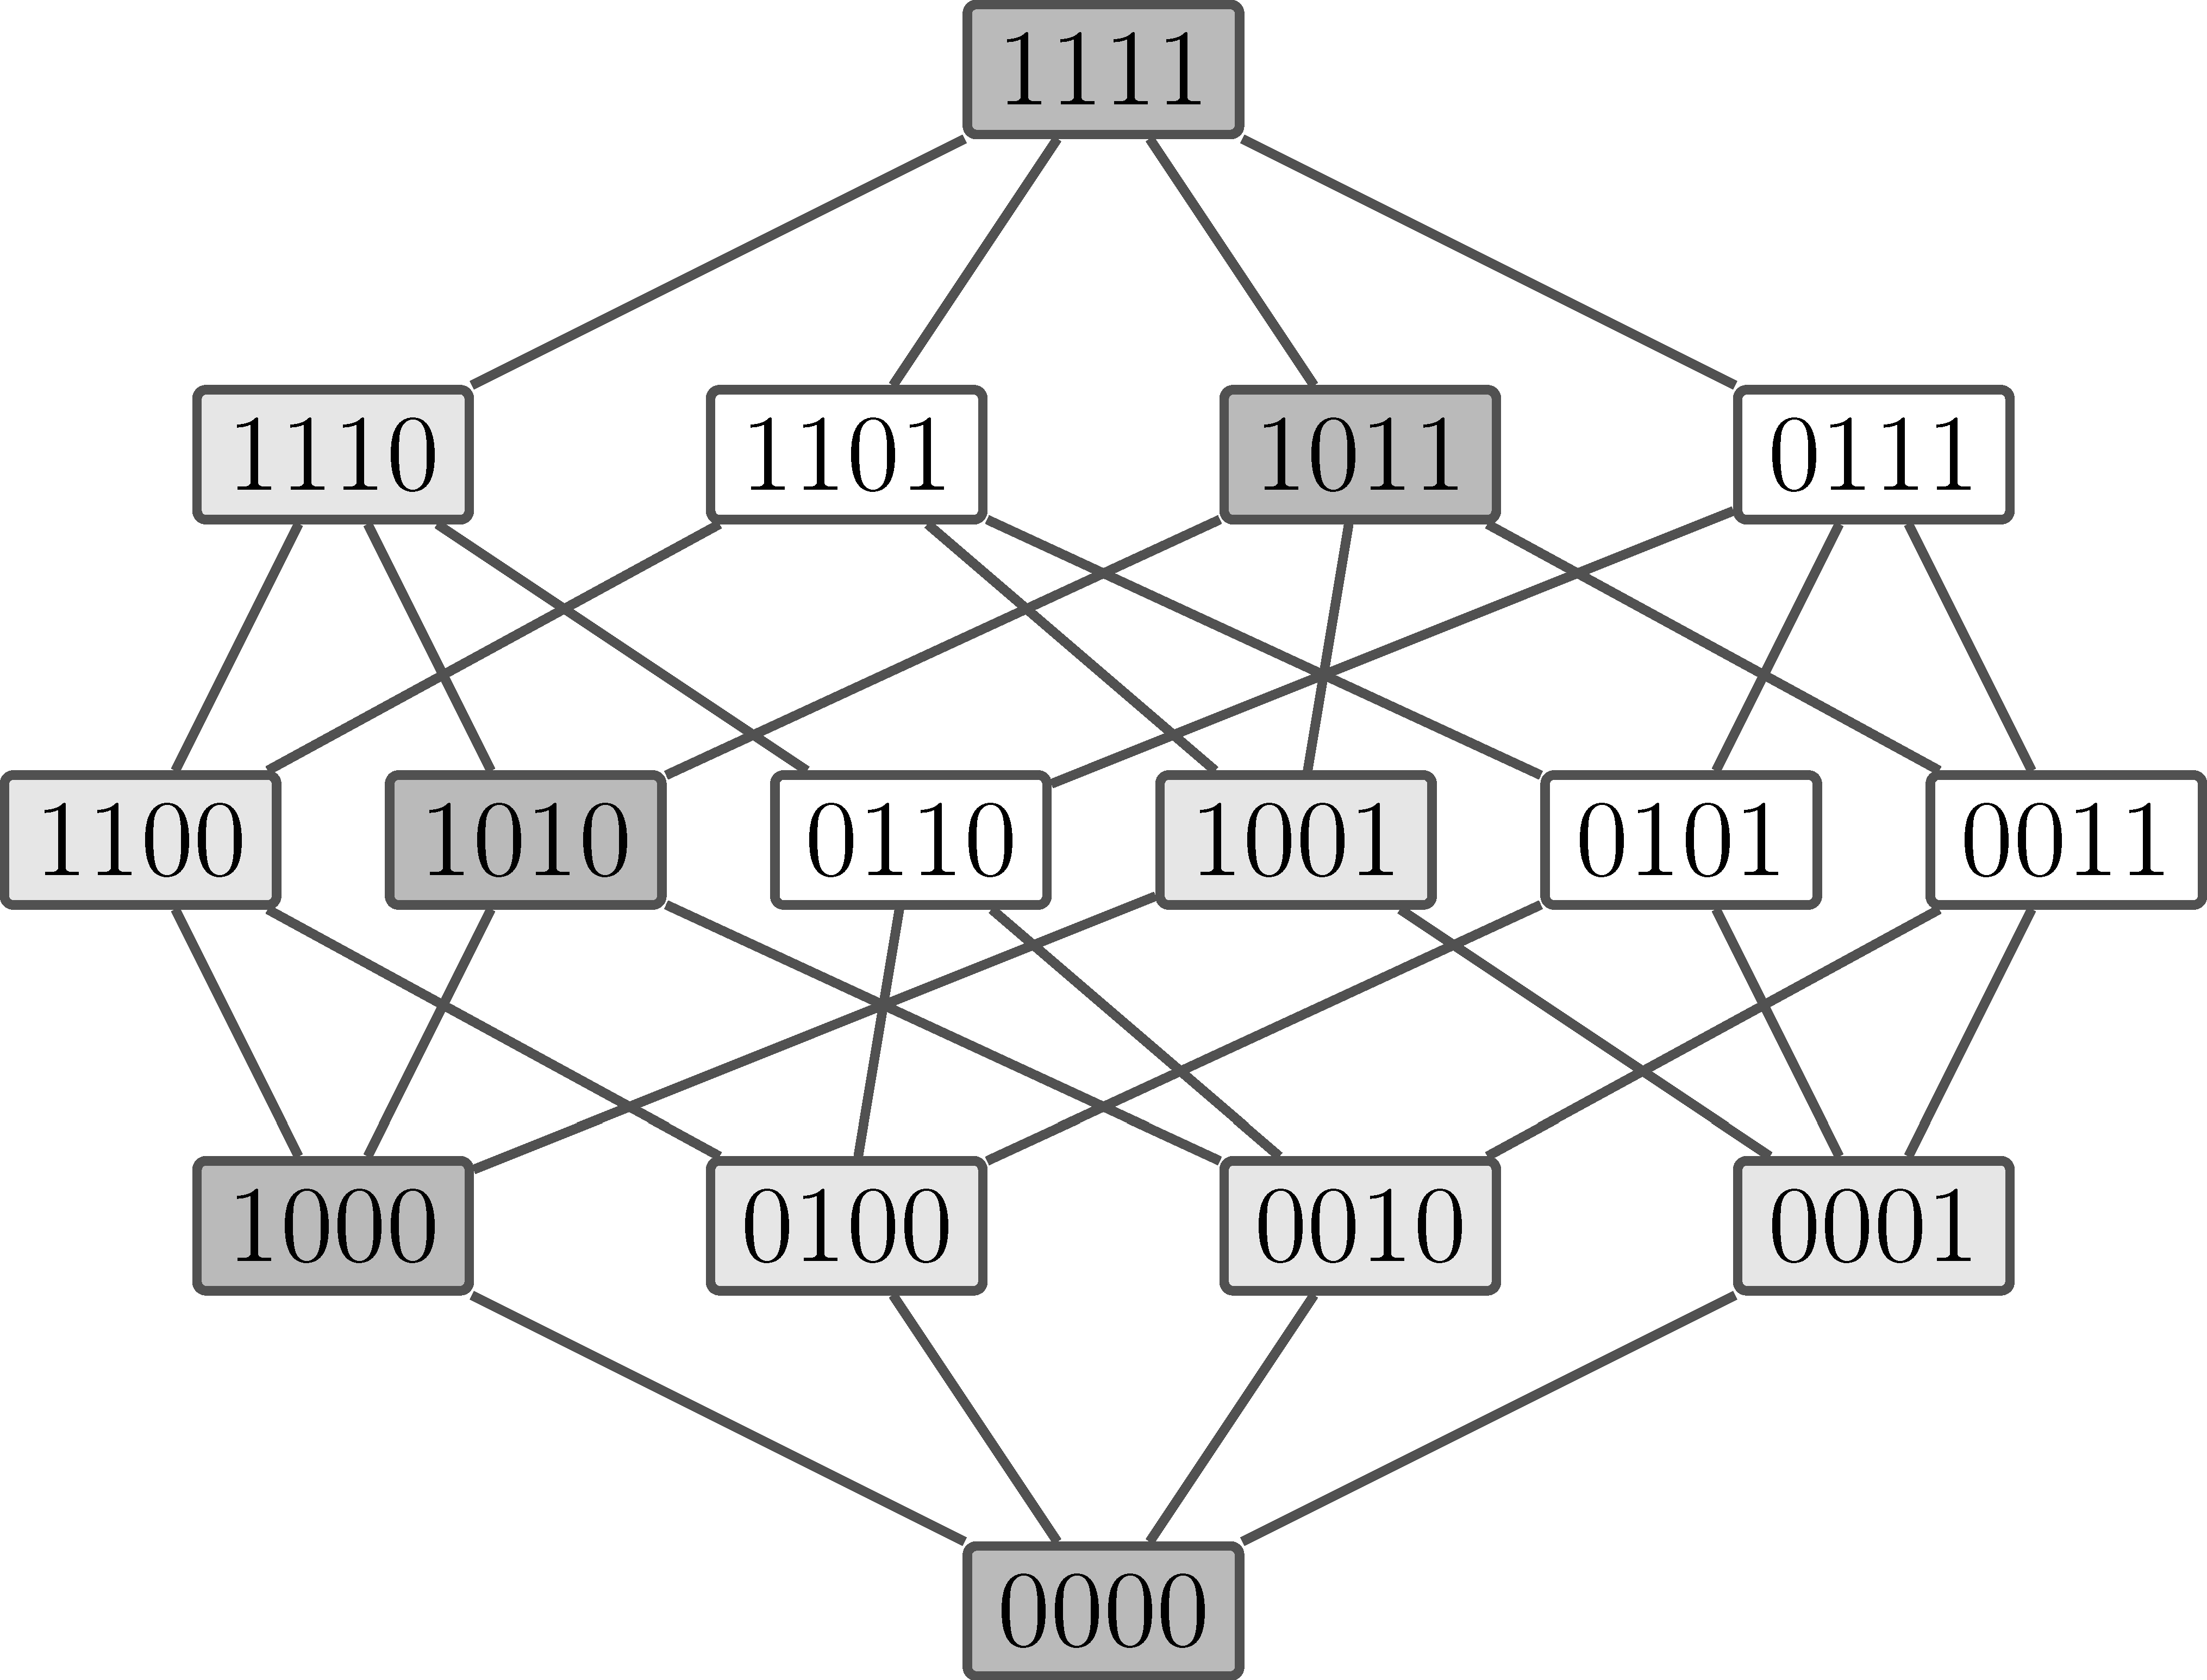
\includegraphics[width=0.8\textwidth,height=\textheight]{chapters/chapter6/Figures/mlr3book_figures-16.png}

}

\caption{\label{fig-sequential-forward-selection}A binary representation
of sequential forward selection with four features. Gray indicates
feature sets that were evaluated, with dark gray indicating the best
feature set in each iteration; white indicates feature sets that were
not evaluated. We start at the bottom with no selected features (all are
`0'). In the next iteration all features are separately tested (each is
`1' separately) and the best option (darkest in row two) is selected.
This continues for selecting the second, third, and fourth features.}

\end{figure}

Wrapper methods can be used with any learner, but need to train or even
resample the learner potentially many times, leading to a
computationally intensive method. All wrapper methods are implemented
via the package
\href{https://mlr3fselect.mlr-org.com}{\texttt{mlr3fselect}}\index{\texttt{mlr3fselect}}.

\begin{tcolorbox}[enhanced jigsaw, opacitybacktitle=0.6, rightrule=.15mm, opacityback=0, arc=.35mm, breakable, titlerule=0mm, colframe=quarto-callout-tip-color-frame, coltitle=black, bottomrule=.15mm, toprule=.15mm, colback=white, colbacktitle=quarto-callout-tip-color!10!white, bottomtitle=1mm, toptitle=1mm, title=\textcolor{quarto-callout-tip-color}{\faLightbulb}\hspace{0.5em}{Feature Selection and HPO}, leftrule=.75mm, left=2mm]

The wrapper-based feature selection explained above is very similar to
the black box optimization approach in HPO
(Chapter~\ref{sec-optimization}), see also
Figure~\ref{fig-optimization-loop-basic}. The major difference is that
we search for well-performing feature subsets instead of hyperparameter
configurations. This similarity is not only true in terms of underlying
concepts and structure, but also with respect to \texttt{mlr3} classes
and API. The API is in many places nearly identical, we can use the same
terminators, results are logged into an archive in a similar fashion to
tuning, and we can also optimize multiple performance measures to create
Pareto-optimal solutions in a similar way

\end{tcolorbox}

\hypertarget{sec-fs-wrapper-example}{%
\subsection{Simple Forward Selection Example}\label{sec-fs-wrapper-example}}

We start with the simple example from above and do sequential forward
selection with \texttt{tsk("penguins")}, similarly to how the sugar
function
\href{https://mlr3tuning.mlr-org.com/reference/tune.html}{\texttt{tune()}}
shown in Section~\ref{sec-autotuner} works, we can use
\href{https://mlr3fselect.mlr-org.com/reference/fselect.html}{\texttt{fselect()}}\index{\texttt{fselect()}}{\marginnote{\begin{footnotesize}\texttt{fselect()}\end{footnotesize}}}
to directly start the optimization and select features.

\begin{Shaded}
\begin{Highlighting}[]
\FunctionTok{library}\NormalTok{(mlr3fselect)}

\CommentTok{\# subset features to ease visualization}
\NormalTok{tsk\_pen }\OtherTok{=} \FunctionTok{tsk}\NormalTok{(}\StringTok{"penguins"}\NormalTok{)}
\NormalTok{tsk\_pen}\SpecialCharTok{$}\FunctionTok{select}\NormalTok{(}\FunctionTok{c}\NormalTok{(}\StringTok{"bill\_depth"}\NormalTok{, }\StringTok{"bill\_length"}\NormalTok{, }\StringTok{"body\_mass"}\NormalTok{,}
  \StringTok{"flipper\_length"}\NormalTok{))}

\NormalTok{instance }\OtherTok{=} \FunctionTok{fselect}\NormalTok{(}
  \AttributeTok{fselector =} \FunctionTok{fs}\NormalTok{(}\StringTok{"sequential"}\NormalTok{),}
  \AttributeTok{task =}\NormalTok{  tsk\_pen,}
  \AttributeTok{learner =}\NormalTok{ lrn\_rpart,}
  \AttributeTok{resampling =} \FunctionTok{rsmp}\NormalTok{(}\StringTok{"cv"}\NormalTok{, }\AttributeTok{folds =} \DecValTok{3}\NormalTok{),}
  \AttributeTok{measure =} \FunctionTok{msr}\NormalTok{(}\StringTok{"classif.acc"}\NormalTok{)}
\NormalTok{)}
\end{Highlighting}
\end{Shaded}

To show all analyzed feature subsets and the corresponding performance,
we use \texttt{as.data.table(instance\$archive)}. In this example, the
\texttt{batch\_nr} column represents the iteration of the sequential
forward selection\index{sequential forward selection} and we start by
looking at the first iteration.

\begin{Shaded}
\begin{Highlighting}[]
\NormalTok{dt }\OtherTok{=} \FunctionTok{as.data.table}\NormalTok{(instance}\SpecialCharTok{$}\NormalTok{archive)}
\NormalTok{dt[batch\_nr }\SpecialCharTok{==} \DecValTok{1}\NormalTok{, }\DecValTok{1}\SpecialCharTok{:}\DecValTok{5}\NormalTok{]}
\end{Highlighting}
\end{Shaded}

\begin{verbatim}
   bill_depth bill_length body_mass flipper_length classif.acc
1:       TRUE       FALSE     FALSE          FALSE      0.7557
2:      FALSE        TRUE     FALSE          FALSE      0.7353
3:      FALSE       FALSE      TRUE          FALSE      0.7064
4:      FALSE       FALSE     FALSE           TRUE      0.7936
\end{verbatim}

We see that the feature \texttt{flipper\_length} achieved the highest
prediction performance in the first iteration and is thus selected. We
plot the performance over the iterations:

\begin{Shaded}
\begin{Highlighting}[]
\FunctionTok{autoplot}\NormalTok{(instance, }\AttributeTok{type =} \StringTok{"performance"}\NormalTok{)}
\end{Highlighting}
\end{Shaded}

\begin{figure}

{\centering 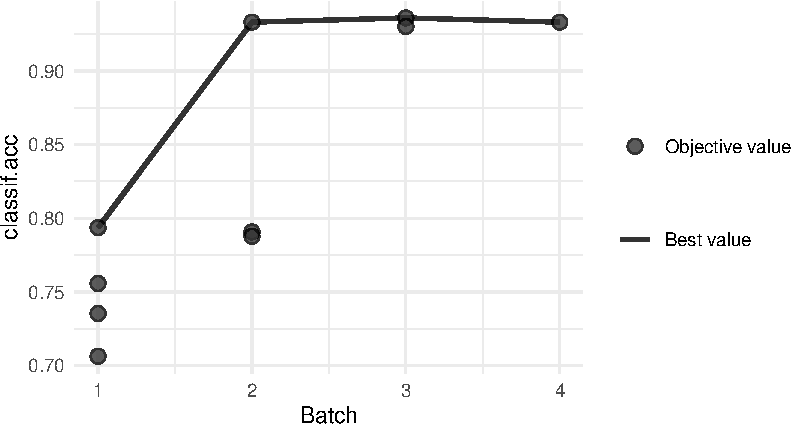
\includegraphics[width=1\textwidth,height=\textheight]{chapters/chapter6/feature_selection_files/figure-pdf/fig-forwardselection-1.pdf}

}

\caption{\label{fig-forwardselection}Model performance in iterations of
sequential forward selection.}

\end{figure}

In the plot, we can see that adding a second feature further improves
the performance to over 90\%. To see which feature was added, we can go
back to the archive and look at the second iteration:

\begin{Shaded}
\begin{Highlighting}[]
\NormalTok{dt[batch\_nr }\SpecialCharTok{==} \DecValTok{2}\NormalTok{, }\DecValTok{1}\SpecialCharTok{:}\DecValTok{5}\NormalTok{]}
\end{Highlighting}
\end{Shaded}

\begin{verbatim}
   bill_depth bill_length body_mass flipper_length classif.acc
1:       TRUE       FALSE     FALSE           TRUE      0.7907
2:      FALSE        TRUE     FALSE           TRUE      0.9331
3:      FALSE       FALSE      TRUE           TRUE      0.7878
\end{verbatim}

The improvement in batch three is small so we may even prefer to select
a marginally worse model with two features to reduce data size.

To directly show the best feature set, we can use
\texttt{\$result\_feature\_set} which returns the features in
alphabetical order (not order selected):

\begin{Shaded}
\begin{Highlighting}[]
\NormalTok{instance}\SpecialCharTok{$}\NormalTok{result\_feature\_set}
\end{Highlighting}
\end{Shaded}

\begin{verbatim}
[1] "bill_depth"     "bill_length"    "flipper_length"
\end{verbatim}

At the heart of \texttt{mlr3fselect} are the R6 classes:

\begin{itemize}
\tightlist
\item
  \texttt{FSelectInstanceSingleCrit},
  \href{https://mlr3fselect.mlr-org.com/reference/FSelectInstanceMultiCrit.html}{\texttt{FSelectInstanceMultiCrit}}:
  These two classes describe the feature selection problem and store the
  results.
\item
  \href{https://mlr3fselect.mlr-org.com/reference/FSelector.html}{\texttt{FSelector}}:
  This class is the base class for implementations of feature selection
  algorithms.
\end{itemize}

Internally, the \texttt{fselect()} function creates an
\href{https://mlr3fselect.mlr-org.com/reference/FSelectInstanceSingleCrit.html}{\texttt{FSelectInstanceSingleCrit}}
object and executes the feature selection with an
\href{https://mlr3fselect.mlr-org.com/reference/FSelector.html}{\texttt{FSelector}}\index{\texttt{FSelector}}
object, based on the selected method, in this example an
\href{https://mlr3fselect.mlr-org.com/reference/mlr_fselectors_sequential.html}{\texttt{FSelectorSequential}}
object. This is similar to what happens in the \texttt{tune()} function
and will be explained in more detail in the following section. It uses
the supplied resampling and measure to evaluate all feature subsets
provided by the \texttt{FSelector} on the task.

In the following two sections, these classes will be created manually,
to learn more about the \texttt{mlr3fselect} package.

\hypertarget{the-fselectinstance-classes}{%
\subsection{The FSelectInstance Classes}\label{the-fselectinstance-classes}}

To create an \texttt{FSelectInstanceSingleCrit} object, we use the sugar
function
\href{https://mlr3fselect.mlr-org.com/reference/fsi.html}{\texttt{fsi()}}\index{\texttt{fsi()}}{\marginnote{\begin{footnotesize}\texttt{fsi()}\end{footnotesize}}}:

\begin{Shaded}
\begin{Highlighting}[]
\NormalTok{instance }\OtherTok{=} \FunctionTok{fsi}\NormalTok{(}
  \AttributeTok{task =}\NormalTok{ tsk\_pen,}
  \AttributeTok{learner =}\NormalTok{ lrn\_rpart,}
  \AttributeTok{resampling =} \FunctionTok{rsmp}\NormalTok{(}\StringTok{"cv"}\NormalTok{, }\AttributeTok{folds =} \DecValTok{3}\NormalTok{),}
  \AttributeTok{measure =} \FunctionTok{msr}\NormalTok{(}\StringTok{"classif.acc"}\NormalTok{),}
  \AttributeTok{terminator =} \FunctionTok{trm}\NormalTok{(}\StringTok{"evals"}\NormalTok{, }\AttributeTok{n\_evals =} \DecValTok{20}\NormalTok{)}
\NormalTok{)}
\end{Highlighting}
\end{Shaded}

Note that we have not selected a feature selection algorithm and thus
did not select any features, yet. We have also supplied a
\texttt{Terminator}, which is used to stop the feature selection, these
are the same objects as we saw in Section~\ref{sec-terminator}.

To start the feature selection, we still need to select an algorithm
which are defined via the
\href{https://mlr3fselect.mlr-org.com/reference/FSelector.html}{\texttt{FSelector}}
class, described in the next section.

\hypertarget{the-fselector-class}{%
\subsection{The FSelector Class}\label{the-fselector-class}}

The \texttt{FSelector}\index{\texttt{FSelector}} class is the base class
for different feature selection algorithms. The following algorithms are
currently implemented in \texttt{mlr3fselect}:

\begin{itemize}
\tightlist
\item
  Random search, trying random feature subsets until termination
  (\texttt{fs("random\_search")})
\item
  Exhaustive search, trying all possible feature subsets
  (\texttt{fs("exhaustive\_search")})
\item
  Sequential search, i.e.~sequential forward or backward selection
  (\texttt{fs("sequential")})
\item
  Recursive feature elimination, which uses a learner's importance
  scores to iteratively remove features with low feature importance
  (\texttt{fs("rfe")})
\item
  Design points, trying all user-supplied feature sets
  (\texttt{fs("design\_points")})
\item
  Genetic search, implementing a genetic algorithm which treats the
  features as a binary sequence and tries to find the best subset with
  mutations (\texttt{fs("genetic\_search")})
\item
  Shadow variable search, which adds permuted copies of all features
  (shadow variables), performs forward selection, and stops when a
  shadow variable is selected (\texttt{fs("shadow\_variable\_search")})
\end{itemize}

Note that all these methods can be stopped (early) with a terminator,
e.g.~an exhaustive search can be stopped after a given number of
evaluations. In this example, we will use a simple random search and
retrieve it from the
\href{https://mlr3fselect.mlr-org.com/reference/mlr_fselectors.html}{\texttt{mlr\_fselectors}}\index{\texttt{mlr\_fselectors}}
dictionary with
\href{https://mlr3fselect.mlr-org.com/reference/fs.html}{\texttt{fs()}}\index{\texttt{fs()}}{\marginnote{\begin{footnotesize}\texttt{fs()}\end{footnotesize}}}.

\begin{Shaded}
\begin{Highlighting}[]
\NormalTok{fselector }\OtherTok{=} \FunctionTok{fs}\NormalTok{(}\StringTok{"random\_search"}\NormalTok{)}
\end{Highlighting}
\end{Shaded}

\hypertarget{starting-the-feature-selection}{%
\subsection{Starting the Feature Selection}\label{starting-the-feature-selection}}

To start the feature selection, we pass the
\texttt{FSelectInstanceSingleCrit} object to the \texttt{\$optimize()}
method of the initialized \texttt{FSelector} object:

\begin{Shaded}
\begin{Highlighting}[]
\NormalTok{fselector}\SpecialCharTok{$}\FunctionTok{optimize}\NormalTok{(instance)}
\end{Highlighting}
\end{Shaded}

The algorithm proceeds as follows

\begin{enumerate}
\def\labelenumi{\arabic{enumi}.}
\tightlist
\item
  The \texttt{FSelector} proposes at least one feature subset or may
  propose multiple subsets to be evaluated in parallel, which can be
  controlled via the setting \texttt{batch\_size}.
\item
  For each feature subset, the given learner is fitted on the task using
  the provided resampling and evaluated with the given measure.
\item
  All evaluations are stored in the archive of the
  \texttt{FSelectInstanceSingleCrit} object.
\item
  The terminator is queried. If the termination criteria are not
  triggered, go to 1).
\item
  Determine the feature subset with the best-observed performance.
\item
  Store the best feature subset as the result in the instance object.
\end{enumerate}

The best feature subset and the corresponding measured performance can
be accessed from the instance:

\begin{Shaded}
\begin{Highlighting}[]
  \FunctionTok{as.data.table}\NormalTok{(instance}\SpecialCharTok{$}\NormalTok{result)[, .(features, classif.acc)]}
\end{Highlighting}
\end{Shaded}

\begin{verbatim}
                               features classif.acc
1: bill_length,body_mass,flipper_length       0.936
\end{verbatim}

As in the forward selection example above, one can investigate all
subset evaluations, which are stored in the archive of the
\texttt{FSelectInstanceSingleCrit} object and can be accessed by using
\texttt{as.data.table()}:

\begin{Shaded}
\begin{Highlighting}[]
\FunctionTok{as.data.table}\NormalTok{(instance}\SpecialCharTok{$}\NormalTok{archive)[}\DecValTok{1}\SpecialCharTok{:}\DecValTok{5}\NormalTok{,}
\NormalTok{  .(bill\_depth, bill\_length, body\_mass, flipper\_length, classif.acc)]}
\end{Highlighting}
\end{Shaded}

\begin{verbatim}
   bill_depth bill_length body_mass flipper_length classif.acc
1:      FALSE        TRUE     FALSE          FALSE      0.7558
2:      FALSE        TRUE     FALSE          FALSE      0.7558
3:      FALSE       FALSE      TRUE          FALSE      0.7210
4:      FALSE        TRUE      TRUE           TRUE      0.9360
5:      FALSE        TRUE      TRUE           TRUE      0.9360
\end{verbatim}

Now the optimized feature subset can be used to subset the task and fit
the model on all observations:

\begin{Shaded}
\begin{Highlighting}[]
\NormalTok{tsk\_pen }\OtherTok{=} \FunctionTok{tsk}\NormalTok{(}\StringTok{"penguins"}\NormalTok{)}

\NormalTok{tsk\_pen}\SpecialCharTok{$}\FunctionTok{select}\NormalTok{(instance}\SpecialCharTok{$}\NormalTok{result\_feature\_set)}
\NormalTok{lrn\_rpart}\SpecialCharTok{$}\FunctionTok{train}\NormalTok{(tsk\_pen)}
\end{Highlighting}
\end{Shaded}

The trained model can now be used to make a prediction on external data.

\hypertarget{sec-multicrit-featsel}{%
\subsection{Optimizing Multiple Performance Measures}\label{sec-multicrit-featsel}}

You might want to use multiple criteria to evaluate the performance of
the feature subsets. With \texttt{mlr3fselect}, the result is the
collection of all feature subsets which are not
Pareto-dominated\index{Pareto optimality} by another subset. Again, we
point out the similarity with HPO and refer to multi-objective
hyperparameter optimization (see Section~\ref{sec-multi-metrics-tuning}
and Karl et al. (2022)).

In the following example, we will perform feature selection on the sonar
dataset. This time, we will use
\href{https://mlr3fselect.mlr-org.com/reference/FSelectInstanceMultiCrit.html}{\texttt{FSelectInstanceMultiCrit}}
to select a subset of features that has high sensitivity, i.e.~TPR, and
high specificity, i.e.~TNR. The feature selection process with multiple
criteria is similar to that with a single criterion, except that we
select two measures to be optimized:

\begin{Shaded}
\begin{Highlighting}[]
\NormalTok{instance }\OtherTok{=} \FunctionTok{fsi}\NormalTok{(}
  \AttributeTok{task =} \FunctionTok{tsk}\NormalTok{(}\StringTok{"sonar"}\NormalTok{),}
  \AttributeTok{learner =}\NormalTok{ lrn\_rpart,}
  \AttributeTok{resampling =} \FunctionTok{rsmp}\NormalTok{(}\StringTok{"holdout"}\NormalTok{),}
  \AttributeTok{measure =} \FunctionTok{msrs}\NormalTok{(}\FunctionTok{c}\NormalTok{(}\StringTok{"classif.tpr"}\NormalTok{, }\StringTok{"classif.tnr"}\NormalTok{)),}
  \AttributeTok{terminator =} \FunctionTok{trm}\NormalTok{(}\StringTok{"evals"}\NormalTok{, }\AttributeTok{n\_evals =} \DecValTok{20}\NormalTok{)}
\NormalTok{)}
\end{Highlighting}
\end{Shaded}

The function
\href{https://mlr3fselect.mlr-org.com/reference/fsi.html}{\texttt{fsi}}
creates an instance of \texttt{FSelectInstanceMultiCrit} if more than
one measure is selected. We now create an
\href{https://mlr3fselect.mlr-org.com/reference/FSelector.html}{\texttt{FSelector}}
and call the \texttt{\$optimize()} function of the \texttt{FSelector}
with the \texttt{FSelectInstanceMultiCrit} object, to search for the
subset of features with the best TPR and FPR. Note that these two
measures cannot both be optimal at the same time (except for the perfect
classifier) and we expect several Pareto-optimal solutions.

\begin{Shaded}
\begin{Highlighting}[]
\NormalTok{fselector }\OtherTok{=} \FunctionTok{fs}\NormalTok{(}\StringTok{"random\_search"}\NormalTok{)}
\NormalTok{fselector}\SpecialCharTok{$}\FunctionTok{optimize}\NormalTok{(instance)}
\end{Highlighting}
\end{Shaded}

As above, the best feature subsets and the corresponding measured
performance can be accessed from the instance.

\begin{Shaded}
\begin{Highlighting}[]
\FunctionTok{as.data.table}\NormalTok{(instance}\SpecialCharTok{$}\NormalTok{result)[, .(features, classif.tpr, classif.tnr)]}
\end{Highlighting}
\end{Shaded}

\begin{verbatim}
                      features classif.tpr classif.tnr
1: V16,V21,V31,V37,V48,V50,...      0.6410      0.8333
2:   V1,V11,V12,V18,V2,V25,...      0.8205      0.7667
3:  V1,V10,V12,V13,V14,V16,...      0.8718      0.7333
4:  V1,V13,V15,V17,V18,V19,...      0.9231      0.6333
\end{verbatim}

We see different tradeoffs of sensitivity and specificity but no feature
subset is dominated by another, i.e.~has worse sensitivity \emph{and}
specificity than any other subset.

\hypertarget{sec-autofselect}{%
\subsection{Nested Resampling}\label{sec-autofselect}}

As in tuning, the performance estimate of the finally selected feature
subset is usually optimistically biased. To obtain unbiased performance
estimates, nested resampling is required and can be set up analogously
to HPO (see Section~\ref{sec-nested-resampling}). We now show this as an
example on the \texttt{sonar} task. The
\href{https://mlr3fselect.mlr-org.com/reference/AutoFSelector.html}{\texttt{AutoFSelector}}\index{\texttt{AutoFSelector}}
class wraps a learner and augments it with automatic feature selection.
Because the \texttt{AutoFSelector} itself inherits from the
\href{https://mlr3.mlr-org.com/reference/Learner.html}{\texttt{Learner}}
base class, it can be used like any other learner. In the example below,
a logistic regression learner is created. This learner is then wrapped
in a random search feature selector that uses holdout (inner) resampling
for performance evaluation. The sugar function
\href{https://mlr3fselect.mlr-org.com/reference/auto_fselector.html}{\texttt{auto\_fselector}}\index{\texttt{auto\_fselector}}{\marginnote{\begin{footnotesize}\texttt{auto\_fselector}\end{footnotesize}}}
can be used to create an instance of \texttt{AutoFSelector}:

\begin{Shaded}
\begin{Highlighting}[]
\NormalTok{afs }\OtherTok{=} \FunctionTok{auto\_fselector}\NormalTok{(}
  \AttributeTok{fselector =} \FunctionTok{fs}\NormalTok{(}\StringTok{"random\_search"}\NormalTok{),}
  \AttributeTok{learner =} \FunctionTok{lrn}\NormalTok{(}\StringTok{"classif.log\_reg"}\NormalTok{),}
  \AttributeTok{resampling =} \FunctionTok{rsmp}\NormalTok{(}\StringTok{"holdout"}\NormalTok{),}
  \AttributeTok{measure =} \FunctionTok{msr}\NormalTok{(}\StringTok{"classif.acc"}\NormalTok{),}
  \AttributeTok{terminator =} \FunctionTok{trm}\NormalTok{(}\StringTok{"evals"}\NormalTok{, }\AttributeTok{n\_evals =} \DecValTok{10}\NormalTok{)}
\NormalTok{)}
\NormalTok{afs}
\end{Highlighting}
\end{Shaded}

\begin{verbatim}
<AutoFSelector:classif.log_reg.fselector>
* Model: list
* Packages: mlr3, mlr3fselect, mlr3learners, stats
* Predict Type: response
* Feature Types: logical, integer, numeric, character, factor,
  ordered
* Properties: loglik, twoclass
\end{verbatim}

The \texttt{AutoFSelector} can then be passed to \texttt{benchmark()} or
\texttt{resample()} for nested resampling
(Section~\ref{sec-nested-resampling}). Below we compare our wrapped
learner \texttt{afs} with a normal logistic regression
\texttt{lrn("classif.log\_reg")}.

\begin{Shaded}
\begin{Highlighting}[]
\NormalTok{grid }\OtherTok{=} \FunctionTok{benchmark\_grid}\NormalTok{(}\FunctionTok{tsk}\NormalTok{(}\StringTok{"sonar"}\NormalTok{), }\FunctionTok{list}\NormalTok{(afs, }\FunctionTok{lrn}\NormalTok{(}\StringTok{"classif.log\_reg"}\NormalTok{)),}
  \FunctionTok{rsmp}\NormalTok{(}\StringTok{"cv"}\NormalTok{, }\AttributeTok{folds =} \DecValTok{3}\NormalTok{))}

\NormalTok{bmr }\OtherTok{=} \FunctionTok{benchmark}\NormalTok{(grid)}\SpecialCharTok{$}\FunctionTok{aggregate}\NormalTok{(}\FunctionTok{msr}\NormalTok{(}\StringTok{"classif.acc"}\NormalTok{))}
\FunctionTok{as.data.table}\NormalTok{(bmr)[, .(learner\_id, classif.acc)]}
\end{Highlighting}
\end{Shaded}

\begin{verbatim}
                  learner_id classif.acc
1: classif.log_reg.fselector      0.7061
2:           classif.log_reg      0.6776
\end{verbatim}

We can see that, in this example, the feature selection improves
prediction performance.

\hypertarget{conclusion-4}{%
\section{Conclusion}\label{conclusion-4}}

In this chapter, we learned how to perform feature selection with
\texttt{mlr3}. We introduced filter and wrapper methods and covered the
optimization of multiple performance measures. Once you have learned
about pipelines we will return to feature selection in
Section~\ref{sec-pipelines-featsel}.

If you are interested in learning more about feature selection then we
recommend an overview of methods in Chandrashekar and Sahin (2014); a
more formal and detailed introduction to filters and wrappers is in
Guyon and Elisseeff (2003), and a benchmark of filter methods was
performed by Bommert et al. (2020).

\hypertarget{tbl-api-feature-selection}{}
\begin{longtable}[]{@{}
  >{\raggedright\arraybackslash}p{(\columnwidth - 4\tabcolsep) * \real{0.3333}}
  >{\raggedright\arraybackslash}p{(\columnwidth - 4\tabcolsep) * \real{0.3333}}
  >{\raggedright\arraybackslash}p{(\columnwidth - 4\tabcolsep) * \real{0.3333}}@{}}
\caption{\label{tbl-api-feature-selection}Important classes and
functions covered in this chapter with underlying class (if applicable),
class constructor or function, and important class fields and methods
(if applicable).}\tabularnewline
\toprule\noalign{}
\begin{minipage}[b]{\linewidth}\raggedright
Class
\end{minipage} & \begin{minipage}[b]{\linewidth}\raggedright
Constructor/Function
\end{minipage} & \begin{minipage}[b]{\linewidth}\raggedright
Fields/Methods
\end{minipage} \\
\midrule\noalign{}
\endfirsthead
\toprule\noalign{}
\begin{minipage}[b]{\linewidth}\raggedright
Class
\end{minipage} & \begin{minipage}[b]{\linewidth}\raggedright
Constructor/Function
\end{minipage} & \begin{minipage}[b]{\linewidth}\raggedright
Fields/Methods
\end{minipage} \\
\midrule\noalign{}
\endhead
\bottomrule\noalign{}
\endlastfoot
\href{https://www.rdocumentation.org/packages/base/topics/funprog}{\texttt{Filter}}
&
\href{https://mlr3filters.mlr-org.com/reference/flt.html}{\texttt{flt()}}
& \texttt{\$calculate()} \\
\href{https://mlr3fselect.mlr-org.com/reference/FSelectInstanceSingleCrit.html}{\texttt{FSelectInstanceSingleCrit}}
or
\href{https://mlr3fselect.mlr-org.com/reference/FSelectInstanceMultiCrit.html}{\texttt{FSelectInstanceMultiCrit}}
&
\href{https://mlr3fselect.mlr-org.com/reference/fselect.html}{\texttt{fselect()}}
& - \\
\href{https://mlr3fselect.mlr-org.com/reference/FSelector.html}{\texttt{FSelector}}
&
\href{https://mlr3fselect.mlr-org.com/reference/fs.html}{\texttt{fs()}}
& \texttt{\$optimize()} \\
\href{https://mlr3fselect.mlr-org.com/reference/AutoFSelector.html}{\texttt{AutoFSelector}}
&
\href{https://mlr3fselect.mlr-org.com/reference/auto_fselector.html}{\texttt{auto\_fselector()}}
& \texttt{\$train()}; \texttt{\$predict()} \\
\end{longtable}

\hypertarget{exercises-4}{%
\section{Exercises}\label{exercises-4}}

\begin{enumerate}
\def\labelenumi{\arabic{enumi}.}
\tightlist
\item
  Compute the correlation filter scores on \texttt{tsk("mtcars")} and
  use the filter to select the five features most strongly correlated
  with the target. Resample \texttt{lrn("regr.kknn")} on both the full
  dataset and the reduced one, and compare both performances based on
  10-fold CV with respect to MSE. NB: Here, we have performed the
  feature filtering outside of CV, which is generally not a good idea as
  it biases the CV performance estimation. To do this properly,
  filtering should be embedded inside the CV via pipelines -- try to
  come back to this exercise after you read
  Chapter~\ref{sec-pipelines-nonseq} to implement this with less bias.
\item
  Apply backward selection to \texttt{tsk("penguins")} with
  \texttt{lrn("classif.rpart")} and holdout resampling by the
  classification accuracy measure. Compare the results with those in
  Section~\ref{sec-fs-wrapper-example} by also running the forward
  selection from that section. Do the selected features differ? Which
  feature selection method reports a higher classification accuracy in
  its \texttt{\$result}?
\item
  There is a problem in the performance comparison in Exercise 2 as
  feature selection is performed on the test-set. Change the process by
  applying forward feature selection with \texttt{auto\_fselector()}.
  Compare the performance to backward feature selection from Exercise 2
  using nested resampling.
\item
  (*) Write a feature selection algorithm that is a hybrid of a filter
  and a wrapper method. This search algorithm should compute filter
  scores for all features and then perform a forward search. But instead
  of tentatively adding all remaining features to the current feature
  set, it should only stochastically try a subset of the available
  features. Features with high filter scores should be added with higher
  probability. Start by coding a stand-alone R method for this search
  (based on a learner, task, resampling, performance measure and some
  control settings). Then, as a stretch goal, see if you can implement
  this as an R6 class inheriting from \texttt{FSelector}.
\end{enumerate}
